%%
%% This is file `./samples/minutes.tex',
%% generated with the docstrip utility.
%%
%% The original source files were:
%%
%% meetingmins.dtx  (with options: `minutes')
%% ----------------------------------------------------------------------
%% 
%% meetingmins - A LaTeX class for formatting minutes of meetings
%% 
%% Copyright (C) 2011-2013 by Brian D. Beitzel <brian@beitzel.com>
%% 
%% This work may be distributed and/or modified under the
%% conditions of the LaTeX Project Public License (LPPL), either
%% version 1.3c of this license or (at your option) any later
%% version.  The latest version of this license is in the file:
%% 
%% http://www.latex-project.org/lppl.txt
%% 
%% Users may freely modify these files without permission, as long as the
%% copyright line and this statement are maintained intact.
%% 
%% ----------------------------------------------------------------------
%% 
\documentclass[11pt]{meetingmins}


\usepackage{hyperref}
\usepackage{tabularx}

% To include images
\usepackage{graphicx}

% text color
\usepackage{xcolor}


%% CONFIG %%
% Default image directory
\graphicspath{{images/}}


\setcommittee{Intégration des nombres complexes et des Unums en Java avec COJAC}

\setmembers{
    Frédéric Bapst (Superviseur),
    Cédric Tâche (Etudiant)
}

\setpresent{
    Frédéric Bapst (Superviseur),
    Cédric Tâche (Etudiant)
}

\setlength{\headheight}{13.6pt}

\date{9 juin 2021}

\begin{document}

\begin {center} {
    \large \textbf {Intégration des nombres complexes et des Unums en Java avec COJAC}
}
\vspace {0.5ex}

PV de la séance du 9 juin 2020 (9h30 - 10h40) via Teams
\end {center} \vspace {1.5em}

\noindent
\textbf{Présents:} Frédéric Bapst, Cédric Tâche

\section{Ordre du jour}
Les points suivants ont été abordés durant la séance:
\begin{hiddenitems}
    \item Validation du PV du 2 juin 2021.
    \item Cahier des charges v1.0
    \item Rapport v0.2
    \item Fonctionnement de COJAC
    \item Planification
\end{hiddenitems}

\section{PV}
\begin{hiddenitems}
    \item Le PV du 2 juin était complet.
\end{hiddenitems}

\section{Cahier des charges}
\begin{hiddenitems}
    \item Certaines phrases peuvent prêter à confusion.
    \item Certaines tâches peuvent être précisées.
    \item D'autres objectifs secondaires peuvent être ajoutés:
    \begin{itemize}
        \item Documentation de COJAC: rédiger de la documentation en anglais ou faire une vidéo.
        \item Comparaison des approches wrappers et behaviours (qui sont décrites plus loin.)
        \item Ajout d'un CI pour vérifier les tests et compiler le JAR.
    \end{itemize}
    \item D'autres améliorations à la base de code existante seraient aussi le bienvenu.
    \item Un jalon pour la démonstration du premier prototype sera ajouté dans la planification.
    \item Les démonstrations seront spécifiées avant la conception des fonctionnalités.
\end{hiddenitems}

\section{Intégration avec COJAC}
\begin{hiddenitems}
    \item COJAC est un agent JAVA qui modifie les classes lorsqu'elles sont chargées par la JVM comme indiqué sur la figure \ref{fig:static_agent}.
    \begin{figure}[ht]
        \centering
        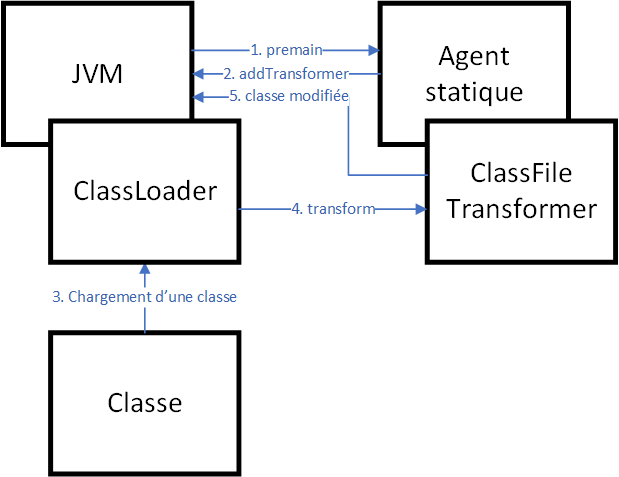
\includegraphics[width=0.7\linewidth]{images/static_agent.png}
        \caption{Principe d'un agent JAVA statique}
        \label{fig:static_agent}
    \end{figure}
    \item COJAC a deux modes de fonctionnement pour changer le comportent des nombres à virgule flottante. Soit le comportement des doubles peut être interprêté différemment (aussi appelé behaviour), soit les doubles peuvent être remplacés par des wrappers.
    \item La réinterprétation des doubles peut se voir dans les classes \textit{BehaviourClassVisitor} et \textit{BehaviourMethodVisitor} ainsi que dans le paquet \textit{models/behaviours}.
    \item Le remplacement des doubles par un wrapper peut se voir dans les classes \textit{FloatReplaceClassVisitor} et \textit{FloatReplaceMethodVisitor} ainsi que dans le paquet \textit{models/wrappers}. Les wrappers \textit{WrapperBasic}, \textit{WrapperBigDecimal} et \textit{WrapperInterval} sont de bons exemples.
    
    \item Les wrappers sont un ensemble de classes hiérarchisées avec un wrapper racine commun.
    \item COJAC a une option \textbf{-W} pour indiquer le type de wrapper à utiliser en remplacement des doubles. Elle permet de tester les wrappers avant d'implémenter l'option spécifique.
\end{hiddenitems}

\section{Erreur COJAC dans les démonstrations}
\begin{hiddenitems}
    \item L'erreur apparaissant pendant l'exécution des démonstrations avec une version de Java supérieure à 8 est due à une nouvelle instruction \textit{invokedynamic} ajoutée dans Java 8 pour supporter les lambdas. Cette instruction a ensuite été utilisée pour d'autres usages dans les versions plus récentes et ces nouvelles utilisations ne sont actuellement pas supportées par COJAC.
\end{hiddenitems}

\section{Autres problèmes avec COJAC}
\begin{hiddenitems}
    \item M. Tâche a remarqué que du code dans COJAC ne respecte pas la documentation de la méthode \textit{transform} qui est disponible au lien suivant: \textcolor{blue}{\url{https://docs.oracle.com/javase/8/docs/api/java/lang/instrument/ClassFileTransformer.html}}. La documentation dit que le tableau retourné doit soit être \textbf{null}, soit être \textbf{un nouveau tableau de bytes}.. A plusieurs endroits, COJAC retourne directement le tableau de bytes d'entrée. Un TODO sera rajouté dans le code, mais la modification ne sera pas forcément faite pendant ce projet.
    \item Le code et l'architecture de COJAC sont très mal documentés. M. Bapst regardera si des anciens rapports d'étudiants contiennent plus d'informations.
\end{hiddenitems}

\section{Librairie de modification du Bytecode JAVA}
\begin{hiddenitems}
    \item La librairie utilisée pour modifier le Bytecode des classes dans le projet se nomme ASM. Cette librairie utilise abondamment le pattern Visitor.
    \item Byte Buddy est une librairie de haut niveau pour générer et modifier des classes depuis un agent Java. Comme ce projet ne nécessitera pas de modifier le Bytecode directement car du code Java est déjà disponible, cette librairie ne sera sûrement pas utilisée. Cependant, c'est une bonne idée de le mentionner dans le rapport, car c'est potentiellement une alternative à ASM.
\end{hiddenitems}

\section{Planification}
\begin{hiddenitems}
    \item Le projet a un retard d'un jour par rapport à la planification dû à des problèmes avec COJAC et des incompréhensions sur son fonctionnement.
\end{hiddenitems}

\section{Décision}
\begin{hiddenitems}
    \item La nouvelle version du cahier des charges sera rendue cette semaine dès que possible.
    \item Le patch de M. Bapst pour corriger l'exécution des démonstrations sera testé avec toutes les démonstrations. Si le résultat est concluant, le patch sera appliqué, sinon la compilation des démonstrations (et des applications utilisateurs) continueront à se faire avec Java 8.
\end{hiddenitems}

\section{Prochaines tâches}
\begin{hiddenitems}
    \item Finir le cahier des charges.
    \item Finir l'analyse de COJAC.
    \item Faire l'analyse des nombres complexes.
    \item Rédiger et coder les spécifications des démonstrations.
    \item Commencer la conception de l'intégration des nombres complexes.
\end{hiddenitems}

\section{Prochaines échéances}
\subsection{Responsable: M. Bapst}

\begin{table}[ht]
    \begin{tabularx}{\columnwidth}{ | X | p{8em} |}
        \hline
        \textbf{Description} & \textbf{Date limite} \\
        \hline
        Chercher les rapports des anciens projets liés à COJAC & 16.06.2021 \\
        \hline
    \end{tabularx}
\end{table}
\subsection{Responsable: M. Tâche}

\begin{table}[ht]
    \begin{tabularx}{\columnwidth}{ | X | p{8em} |}
        \hline
        \textbf{Description} & \textbf{Date limite} \\
        \hline
        Finir le cahier des charges & 11.06.2021 \\
        \hline
    \end{tabularx}
\end{table}

\vspace{1em}
\par \noindent \textbf {Prochaine séance:} Le mercredi 16 juin 2020 à 9h30

\end{document}
%% 
%% Copyright (C) 2011-2013 by Brian D. Beitzel <brian@beitzel.com>
%% 
%% This work may be distributed and/or modified under the
%% conditions of the LaTeX Project Public License (LPPL), either
%% version 1.3c of this license or (at your option) any later
%% version.  The latest version of this license is in the file:
%% 
%% http://www.latex-project.org/lppl.txt
%% 
%% Users may freely modify these files without permission, as long as the
%% copyright line and this statement are maintained intact.
%% 
%% This work is "maintained" (as per LPPL maintenance status) by
%% Brian D. Beitzel.
%% 
%% This work consists of the file  meetingmins.dtx
%% and the derived files           meetingmins.cls,
%%                                 sampleminutes.tex,
%%                                 department.min,
%%                                 README.txt, and
%%                                 meetingmins.pdf.
%% 
%%
%% End of file `./samples/minutes.tex'.
